%% For double-blind review submission
\documentclass[acmlarge,anonymous]{acmart}\settopmatter{printfolios=true} % review will add line numbers -- anonymous will make it anonymous
%% For single-blind review submission
%\documentclass[acmlarge,review]{acmart}\settopmatter{printfolios=true}
%% For final camera-ready submission
%\documentclass[acmlarge]{acmart}\settopmatter{}
\usepackage{wrapfig}
\usepackage[inline]{enumitem}
\usepackage{bussproofs}
\usepackage{bussproofs}
\usepackage{dsfont}
\usepackage{xspace}
\usepackage{mathtools}
\usepackage{amsthm}
\usepackage{mathpartir}
\usepackage{listings}
\usepackage{color}

\usepackage[T1]{fontenc}
\usepackage[utf8]{inputenc}
\usepackage{listings}

\usepackage{xcolor}   % for coloring as emph
\usepackage{etoolbox} % for \ifnumcomp
\usepackage{beramono} % a tt font that has a boldface series
\definecolor{dkgreen}{rgb}{0,0.6,0}
\definecolor{gray}{rgb}{0.5,0.5,0.5}
\definecolor{mauve}{rgb}{0.58,0,0.82}
\lstset{
frame=none,
  language=Java,
  aboveskip=1mm,
  belowskip=1mm,
  showstringspaces=false,
  columns=flexible,
  basicstyle={\footnotesize\ttfamily},
  numbers=none,
  numberstyle=\tiny\color{gray},
  keywordstyle=\color{blue},
  commentstyle=\color{dkgreen},
  stringstyle=\color{mauve},
  breaklines=true,
  breakatwhitespace=true,
  tabsize=2}
% The style to be applied for the highlighted line:
\lstdefinestyle{highlight}{basicstyle=\footnotesize\ttfamily \color{red}, keywordstyle=\color{red}}
%\lstdefinestyle{highlight}{backgroundcolor=\color{orange!30}}

% input listing and emphasize a specific line
% \lstinputemph[listings options]{line number}{filename}
\newcommand{\lstinputemph}[3][\empty]{%                                                    
 \lstset{aboveskip=0pt, belowskip=0pt, showlines=true,#1}%
 \ifnumcomp{#2}{=}{0}{\lstinputlisting{#3}}{%
   \ifnumcomp{#2}{=}{1}{}{\lstinputlisting[lastline=\the\numexpr#2-1\relax]{#3}}%            
   \lstinputlisting[firstnumber={#2},firstline={#2},lastline={#2},style=highlight]{#3}
   \lstinputlisting[firstnumber={\the\numexpr#2+1},firstline=\the\numexpr#2+1\relax]{#3}
 }% else
}



%% Note: Authors migrating a paper from PACMPL format to traditional
%% SIGPLAN proceedings format should change 'acmlarge' to
%% 'sigplan,10pt'.

\usepackage{lipsum}  
%% Some recommended packages.
\usepackage{booktabs}   %% For formal tables:
                        %% http://ctan.org/pkg/booktabs
\usepackage{subcaption} %% For complex figures with subfigures/subcaptions
                        %% http://ctan.org/pkg/subcaption


\makeatletter\if@ACM@journal\makeatother
%% Journal information (used by PACMPL format)
%% Supplied to authors by publisher for camera-ready submission
\acmJournal{PACMPL}
\acmVolume{1}
\acmNumber{1}
\acmArticle{1}
\acmYear{2017}
\acmMonth{1}
\acmDOI{10.1145/nnnnnnn.nnnnnnn}
\startPage{1}
\else\makeatother
%% Conference information (used by SIGPLAN proceedings format)
%% Supplied to authors by publisher for camera-ready submission
\acmConference[OOPSLA'17]{The ACM SIGPLAN conference on Systems, Programming, Languages and Applications}{January 01--03, 2017}{New York, NY, USA}
\acmYear{2017}
\acmISBN{978-x-xxxx-xxxx-x/YY/MM}
\acmDOI{10.1145/nnnnnnn.nnnnnnn}
\startPage{1}
\fi


%% Copyright information
%% Supplied to authors (based on authors' rights management selection;
%% see authors.acm.org) by publisher for camera-ready submission
\setcopyright{none}             %% For review submission
%\setcopyright{acmcopyright}
%\setcopyright{acmlicensed}
%\setcopyright{rightsretained}
%\copyrightyear{2017}           %% If different from \acmYear


%% Bibliography style
\bibliographystyle{ACM-Reference-Format}
%% Citation style
%% Note: author/year citations are required for papers published as an
%% issue of PACMPL.
\citestyle{acmauthoryear}   %% For author/year citations


%%% New Definitions %%%%%%%
%% -----------------------
\newcommand{\tool}[0]{{\sc syncope}\xspace} % short for SYNthesizing
% COnsistency Property Enforcement.
\newcommand{\conj}{~\wedge~}

\newcommand{\HA}{{\sf HA}}
\newcommand{\SA}{{\sf SA}}
\newcommand{\UA}{{\sf UA}}
\newcommand{\scc}{\psi_{\sf sc}}
\newcommand{\ccc}{\psi_{\sf cc}}
\newcommand{\ecc}{\psi_{\sf ec}}
\newcommand{\rcc}{\psi_{\sf rc}}
\newcommand{\mavc}{\psi_{\sf mav}}
\newcommand{\rrc}{\psi_{\sf rr}}
%\newcommand{\coloneqq}{::=}
\newcommand{\spc}{\quad}

% \newtheorem{theorem}{Theorem}
% \newtheorem{lemma}[theorem]{Lemma}
% \newtheorem{proposition}[theorem]{Proposition}
% \newtheorem{corollary}[theorem]{Corollary}
% \newtheorem{definition}[theorem]{Definition}
% \newcounter{hno}
%   \newcounter{gno}
% \renewenvironment{proof}{\setcounter{hno}{0}\setcounter{gno}{0}
%   \emph{Proof.}}{}
% \newcommand{\npp}{\thehno \stepcounter{hno}}
% \newcommand{\mpp}{\thegno \stepcounter{gno}}

\newcommand{\stretcharraybig}{\renewcommand*{\arraystretch}{1.25}}
\newcommand{\cureff}{\hat{\eta}}
\newcommand{\eff}{\eta}
\newcommand{\fresh}{\N{\sf fresh}}
\newcommand{\cv}{\psi}
\newcommand{\ALT}{~\mid~}
\newcommand{\eid}{{\iota}}
\newcommand{\ObjType}{{\sf ObjType}}
\newcommand{\AbsType}{{\sf AbsType}}
\newcommand{\dom}{{\sf dom}}
\newcommand{\DtLib}[1]{\mathbb{D}(#1)}
\newcommand{\DtLibZ}{\mathbb{D}}
\newcommand{\Ops}{\Lambda}
\newcommand{\Ctrts}{\Psi}
\newcommand{\true}{\N{\textsf{true}}}

\newcommand{\R}[1]{\textrm{#1}}
\newcommand{\N}[1]{{\normalfont #1}}
\newcommand{\ObjZ}{\N{\textsf{Obj}}}
\newcommand{\Obj}[1]{\N{\textsf{Obj}_{#1}}}
\newcommand{\ReplID}{\mathtt{ReplID}}
\newcommand{\SessID}{\mathtt{SessID}}
\newcommand{\typeFun}[1]{\N{\textsf{type}}(#1)}
\newcommand{\Op}[1]{\N{\textsf{Op}_{#1}}}
\newcommand{\set}[1]{\mathcal{P}(#1)}
\newcommand{\unitVal}{\N{\textsf{unit}}}
\newcommand{\EffUniv}{\N{\sf Effect}}
\newcommand{\EffID}{\mathtt{SeqNo}}
\newcommand{\TransID}{\N{\sf TransID}}
\newcommand{\AVal}[1]{\N{\textsf{AVal}_{#1}}}
\newcommand{\RVal}[1]{\N{\textsf{RVal}_{#1}}}
\newcommand{\Eff}[1]{\N{\textsf{Eff}_{#1}}}
\newcommand{\loud}[1]{\textbf{\textit{#1}}}
\newcommand{\dt}[1]{\mathcal{D}_{#1}}
\newcommand{\vis}[2]{\N{\textsf{vis}(#1,#2)}}
\newcommand{\visZ}{\N{\textsf{vis}}}
\newcommand{\depsZ}{\N{\textsf{deps}}}
\newcommand{\deps}[1]{\N{\textsf{deps}(#1)}}
\newcommand{\Rvis}{\N{\textsf{vis}}}
\newcommand{\arZ}{\N{\textsf{ar}}}
\newcommand{\ar}[2]{\N{\textsf{ar}(#1,#2)}}
\newcommand{\stxZ}{\sim}
\newcommand{\stx}[2]{#1\sim#2}
\newcommand{\nstx}[2]{#1\not\sim#2}
\newcommand{\comZ}{\N{\textsf{com}}}
\newcommand{\com}[1]{\comZ(#1)}
\newcommand{\so}[2]{\N{\textsf{so}(#1,#2)}}
\newcommand{\soZ}{\N{\textsf{so}}}
\newcommand{\stZ}{\N{\textsf{st}}}
\newcommand{\Rso}{\N{\textsf{so}}}
\newcommand{\Rst}{\N{\textsf{st}}}
\newcommand{\COM}{\textrm{\sc {\small Commit}}}
\newcommand{\soo}[2]{\N{\textsf{soo}(#1,#2)}}
\newcommand{\sooZ}{\N{\textsf{soo}}}
\newcommand{\hb}[2]{\N{\textsf{hb}(#1,#2)}}
\newcommand{\hbo}[2]{\N{\textsf{hbo}(#1,#2)}}
\newcommand{\hbZ}{\N{\textsf{hb}}}
\newcommand{\hboZ}{\N{\textsf{hbo}}}
\newcommand{\txnZ}{\N{\textsf{txn}}}
\newcommand{\txn}[2]{\txnZ\{#1\}\{#2\}}
\newcommand{\sameobj}[2]{\N{\textsf{sameobj}(#1,#2)}}
\newcommand{\sameobjZ}{\N{\textsf{sameobj}}}
\newcommand{\sametxn}[2]{\N{\textsf{sametxn}(#1,#2)}}
\newcommand{\sametxnZ}{\N{\textsf{sametxn}}}
\newcommand{\E}{\N{\textsf{E}}}
\newcommand{\Pool}{\N{\textsf{pool}}}
\newcommand{\Cache}{\N{\textsf{cache}}}
\newcommand{\Avail}{\N{\textsf{avail}}}
\newcommand{\CacheFinder}{\N{\textsf{Ctxt}}}
\newcommand{\EffSoup}{\N{\textsf{A}}}
\newcommand{\obj}{\N{\textsf{obj}}}
\newcommand{\dep}{\N{\textsf{dep}}}
\newcommand{\ssn}{\N{\textsf{ssn}}}
\newcommand{\id}{\N{\textsf{id}}}
\newcommand{\oper}{\N{\textsf{oper}}}
\newcommand{\rval}{\N{\textsf{rval}}}
\newcommand{\repl}{\N{\textsf{repl}}}
\newcommand{\sess}{\N{\textsf{sess}}}
\newcommand{\rdtspec}{\Delta}
\newcommand{\goesto}{\longrightarrow}
\newcommand{\tuplee}[1]{\langle #1 \rangle}
\newcommand{\ctxtFn}{\N{\textsf{ctxt}}}
\newcommand{\rdtredsto}{\N{\leadsto}}
\newcommand{\Exec}{\N{\textsf{(\EffSoup,\allowbreak \visZ,\allowbreak \soZ)}}}
\newcommand{\pll}{~\|~}
\newcommand{\Mod}[1]{\N{\textsf{Mod}}(#1)}
\newcommand{\De}[1]{#1}
\newcommand{\Der}[2]{[\![#1,#2]\!]_{r}}
\newcommand{\msentails}[2]{#1 \models #2}
\newcommand{\hasTyp}[2]{#1 \vdash #2}
\newcommand{\auxred}[4]{#1 \vdash #2 \xhookrightarrow{#3} #4 }
\renewcommand{\qed}{\nobreak \ifvmode \relax \else
      \ifdim\lastskip<1.5em \hskip-\lastskip
      \hskip1.5em plus0em minus0.5em \fi \nobreak
      \vrule height0.75em width0.5em depth0.25em\fi}


% Operational semantics rules
\newcommand{\rulelabel}[1]{\textrm{\sc {\small [#1]}}}
\newcommand{\RULE}[3]
{\frac{\begin{array}{c}#1\end{array}}
		 {\begin{array}{c}#2\end{array}}
~ \rulelabel{#3}
}

\newcommand{\RuleTwo}[2]
{\frac{\begin{array}{c}#1\end{array}}
		 {\begin{array}{c}#2\end{array}}
}

\newenvironment{nop}{}{}
\newenvironment{smathpar}{
\begin{nop}\small\begin{mathpar}}{
\end{mathpar}\end{nop}\ignorespacesafterend}

\newenvironment{cmathpar}{
\vspace{-3mm}
\renewcommand{\arraystretch}{1.2}
\begin{nop}\begin{mathpar}}{
\end{mathpar}\end{nop}\ignorespacesafterend}

\newcommand{\rsf}[1]{\R{\sf #1}}
\newcommand{\trans}[4]{\N{\textsf{trans}}\{#1,#2\}\{#3,#4\}}

\setlength{\floatsep}{5pt}
\setlength{\textfloatsep}{10pt}
\setlength{\dblfloatsep}{5pt}
\setlength{\dbltextfloatsep}{10pt}


\newcommand{\ecds}{ECDS\xspace}
%\newcommand{\nexists}{\not\exists}
%\newcommand{\nsucc}{\not\succ}


\begin{document}

%% Title information
\title{\tool: Automatic Enforcement of Distributed Consistency Guarantees}         %% [Short Title] is optional;
                                        %% when present, will be used in
                                        %% header instead of Full Title.
%\titlenote{with title note}             %% \titlenote is optional;
                                        %% can be repeated if necessary;
                                        %% contents suppressed with 'anonymous'
%\subtitlenote{with subtitle note}       %% \subtitlenote is optional;
                                        %% can be repeated if necessary;
                                        %% contents suppressed with 'anonymous'


%% Author information
%% Contents and number of authors suppressed with 'anonymous'.
%% Each author should be introduced by \author, followed by
%% \authornote (optional), \orcid (optional), \affiliation, and
%% \email.
%% An author may have multiple affiliations and/or emails; repeat the
%% appropriate command.
%% Many elements are not rendered, but should be provided for metadata
%% extraction tools.

% FIRST AUTHOR
%% Author with single affiliation.
\author{Kia Rahmani}
%\authornote{with author1 note}          %% \authornote is optional;
                                        %% can be repeated if necessary
\orcid{nnnn-nnnn-nnnn-nnnn}             %% \orcid is optional
\affiliation{
  \position{PhD Student}
  \department{Computer Science}              %% \department is recommended
  \institution{Purdue University}            %% \institution is required
  \streetaddress{Street1 Address1}
  \city{City1}
  \state{State1}
  \postcode{Post-Code1}
  \country{Country1}
}
\email{rahmank@purdue.edu}          %% \email is recommended
%------------------------------------------------------------------------------------
%SECOND AUTHOR
\author{Gowtham Kaki}
%\authornote{with author1 note}          %% \authornote is optional;
                                        %% can be repeated if necessary
\orcid{nnnn-nnnn-nnnn-nnnn}             %% \orcid is optional
\affiliation{
  \position{PhD Student}
  \department{Computer Science}              %% \department is recommended
  \institution{Purdue University}            %% \institution is required
  \streetaddress{Street1 Address1}
  \city{City1}
  \state{State1}
  \postcode{Post-Code1}
  \country{Country1}
}
\email{rahmank@purdue.edu}       


%------------------------------------------------------------------------------------
%THIRD AUTHOR
\author{Suresh Jagannathan}
%\authornote{with author1 note}          %% \authornote is optional;
                                        %% can be repeated if necessary
\orcid{nnnn-nnnn-nnnn-nnnn}             %% \orcid is optional
\affiliation{
  \position{PhD Student}
  \department{Computer Science}              %% \department is recommended
  \institution{Purdue University}            %% \institution is required
  \streetaddress{Street1 Address1}
  \city{City1}
  \state{State1}
  \postcode{Post-Code1}
  \country{Country1}
}
\email{rahmank@purdue.edu}   
%------------------------------------------------------------------------------------


%% Paper note
%% The \thanks command may be used to create a "paper note" ---
%% similar to a title note or an author note, but not explicitly
%% associated with a particular element.  It will appear immediately
%% above the permission/copyright statement.
%\thanks{with paper note}                %% \thanks is optional
                                        %% can be repeated if necesary
                                        %% contents suppressed with 'anonymous'


%% Abstract
%% Note: \begin{abstract}...\end{abstract} environment must come
%% before \maketitle command

\begin{abstract}

  Modern-day distributed systems often use replication to improve
  communication latency and fault tolerance among geographically
  distributed servers and clients.  But, replication compromises
  simplicity because it forces applications to weigh the correctness
  benefits of guaranteeing strong consistency against a potentially
  significant cost in performance.  Because not all operations on a
  replicated data type require strongly consistent behavior, however,
  library designers should be able to ideally direct implementations
  to provide precisely the level of consistency needed, eschewing the
  costs of strong consistency except when absolutely necessary.
  Unfortunately, implementations typically support only a small set of
  consistency levels.  Consequently, developers must either be content
  with mapping application requirements to a supported consistency
  level that may well enforce stronger guarantees than required, or
  hand weave a specialized protocol that more accurately matches
  application needs.  The former approach sacrifices performance,
  while the latter entails added complexity.

  In this paper, we describe a lightweight runtime system for weakly
  consistent distributed systems that dynamically customizes a
  consistency protocol based on a declarative axiomatic specification
  that reflects the necessary constraints any correct implementation
  must satisfy.  Our technique generates a provably optimal runtime
  enforcement mechanism that imposes no additional communication or
  blocking overhead beyond what is required to satisfy the
  specification, thus freeing developers from writing bespoke and
  complex consistency protocols without having to sacrifice
  availability and performance by not doing so.

  We demonstrate the applicability of our approach by automatically
  deriving enforcement mechanisms for various well-known weak
  consistency instantiations.  Experimental results show that the
  performance of our automically derived mechanisms is comparable to
  specialized hand-written protocols, providing strong evidence of its
  practical utility.

\end{abstract}


%% 2012 ACM Computing Classification System (CSS) concepts
%% Generate at 'http://dl.acm.org/ccs/ccs.cfm'.
%\begin{CCSXML}
%<ccs2012>
%<concept>
%<concept_id>10011007.10011006.10011008</concept_id>
%<concept_desc>Software and its engineering~General programming languages</concept_desc>
%<concept_significance>500</concept_significance>
%</concept>
%<concept>
%<concept_id>10003456.10003457.10003521.10003525</concept_id>
%<concept_desc>Social and professional topics~History of programming languages</concept_desc>
%<concept_significance>300</concept_significance>
%</concept>
%</ccs2012>
%\end{CCSXML}

%\ccsdesc[500]{Software and its engineering~General programming languages}
%\ccsdesc[300]{Social and professional topics~History of programming languages}
%% End of generated code


%% Keywords
%% comma separated list
%\keywords{Fine Grained Consistency , keyword2, keyword3}  %% \keywords is optional


%% \maketitle
%% Note: \maketitle command must come after title commands, author
%% commands, abstract environment, Computing Classification System
%% environment and commands, and keywords command.
\maketitle

%================================ SECTION ONE
\section{Introduction}
\paragraph{} Most of the modern web-based applications are implemented as
multiple agents simultaneously serving users and working on replicated data objects across 
geographically distributed machines. Implementation and reasoning techniques for strongly 
consistent replicated data stores (e.g. stores providing linearizability and serializability) have been 
studied for decades. 
However, these strong notions of consistency come with the price of availability and low response-
time, which are intrinsically crucial for distributed large-scale applications. Weak consistency models 
such as \emph{monotonic reads} and \emph{monotonic writes} however, liberate the application 
instances from extensive synchronization and allows them to be "always-on" despite of possible 
network partitionings. 
Unfortunately, these weak guarantees suffer from the lack of standardized definitions and 
enforcement methodologies, which forces developers to modify their applications with ad-hoc 
fixes in order to enforce their desired levels of consistency. 
\\ The ad-hoc implementation approaches and the lack of a general reasoning 
framework for weak consistency, has resulted in the difficulty of proving correctness and 
optimality properties of such highly error-prone implementations. To make the matter worse, 
many of distributed applications simultaneously require different levels of consistency for 
different tasks and even face new consistency requirements after the development phase is over. 
\paragraph{} Let's consider a distributed bulletin board application where users send 
requests to servers to post a message or read the current messages on the board. Since the 
underlying data store provides eventual consistency guarantee, we can be sure that every 
message submitted to any server, will \emph{eventually} become visible at all servers. 
However, we might also be interested in ensuring users that if they see a message as a result of a 
read request, they will also see that message in their subsequent reads. This requirement which is 
known as "monotonic reads", is not guaranteed under eventual consistency, since users might 
send read request to different servers with different sets of available messages. 
Version vectors and similar ad-hoc approaches are usually used to add guards to the code in 
order to enforce the required consistency guarantees. This error-prone task requires 
developers to also come up their own proofs of correctness which to make the 
matter worse, has to be renewed each time the application is updated or the 
consistency requirements are changed (e.g. write operations are also realized 
to require guards before executions). 

%The Figure Containing The Bulletin Board and its Modified Version
\begin{figure}[h]
    \centering
    \begin{subfigure}[b]{0.48\textwidth} 
       \lstinputemph[language=Java]{0}{../Introduction/app1.java}
       \label{fig:app1}
    \end{subfigure} ~
       \begin{subfigure}[b]{0.52\textwidth} 
        \lstinputemph[language=Java]{3}{../Introduction/app2.java}
        \label{fig:app2}
    \end{subfigure}\\
    \hrulefill
    \caption{A Bulletin Board Application (left) and the Modified Version Including Guards (right) }
\end{figure}


In this paper, we address these issues by introducing a principled approach to 
derive enforcement mechanisms for various forms of weak consistency 
guarantees. We offer developers with a language to specify their application-level consistency 
requirements as logical formulae expressing allowed relationships between update effects. 
We also introduce a new tool that generates a shim layer on top of the eventually 
consistent data store, and extends it to a key-value store with multiple environments, each of which 
shows the desired behavior specified by the given specifications. Our consistency enforcement 
methodology is independent of the underlying store, and only assumes the well established 
guarantee of "eventual delivery". 
Moreover, our specification language is also powerful enough to express all the known consistency 
guarantees in the context. 

We argue that all the consistency guarantees basically specify, \emph{when} an 
application instance should block a user request and for arrival of 
\emph{what} remote updates it should wait. For obvious reasons, any implementation of these 
consistency guarantees must be \emph{correct} and \emph{optimal}. The former property states that 
all possible behaviors of the implementation are allowed by the given specification and the later 
ensures that application instances do not engage in 
any unnecessary synchronization before responding to a user request (i.e. users are only blocked if 
it is absolutely necessary).
\\ Our technique is based on tracking relationships between update effects, and maintaining multiple 
(logical) caches at the shim layer, each of which is enforced to satisfy a specific level of consistency, 
derived from the given specifications. We believe that our approach is the first ever principled 
reasoning and implementation framework for weak consistency enforcement techniques which 
is also proven to be \emph{correct} and \emph{optimal}. 
By separating all the consistency management procedures from the application level, we are taking 
the non-trivial task of proving soundness criteria for ad-hoc consistency enforcement techniques 
off of the developer's shoulders. 
% Contributions of the paper
\\The paper makes the following contributions:
\begin{itemize}
\item Introducing a new specification language that covers all the known consistency guarantees in 
the context. Our language is arguably simpler than the previous works, and is based on observing 
similarities of different consistency requirements.

\item Proposing a principled consistency enforcement methodology that is 
complete for our specification language and allows deriving multi-purpose consistency enforcement 
tools.

\item Presenting proofs of correctness and optimality of our consistency enforcement methodology 
and introducing the first ever general reasoning framework for weak consistency guarantees. 

\item Introducing our tool called  \tool that realizes our consistency enforcement methods and 
extends an off-the-shelf eventually consistent data store (Cassandra) to a multi purpose key-value 
data store with the ability to guarantee any requested consistency level defined by the 
developers. 

\item Presenting the evaluation results showing the utility of \tool compared to a hard-coded
implementation of a weak consistency guarantee. 
\end{itemize}

% Structure of the paper
The rest of the paper is structured as follows. 
In section 2 we introduce the running example and explain problems associated with it. 
Section 3 introduces our system model, including the distributed underlying database model, our 
multi-purpose shim layer, and the formal definition of our specification language.
In section 4, we introduce our consistency enforcement strategy in detail and introduce the 
formal semantics of the shim layer. In section 5, we present the formal definitions 
and proofs of correctness of optimality properties of our shim. Sections 6 introduces our tool 
including 
the implementation details,  
which is followed by section 7, where the test results from running \tool on 
distributed real world machines are presented. 
We discuss the related works and future directions in the section 8. 


%================================ SECTION TWO
%\section{Motivation}

\newpage
%================================ SECTION FOUR
\section{Formalization}
In this section we first present our specification language and then
introduce the opeational semantics of our tool. The operational semantics of our tool is presented in two different sets. First set of rules, presents the core of our algorithm and we use it to present the proofs of correctness and optimality. 

\subsection{Specification Language}
Following is the formal syntax of contract language in our system:
\begin{figure}[t]
\begin{subfigure}{0.41\textwidth}
\centering
  \begin{fmathpar}
  \begin{array}{lclcl}
		\rel & \in & \texttt{rel.seed} & \coloneqq & \visZ \ALT
		\soZ \ALT \rel \cup \rel \\
               \Rel & \in & \texttt{relation} & \coloneqq &  \rel
	       \ALT \Rel;\rel  \ALT \nullR  \\
	     \pi & \in & \texttt{prop} & \coloneqq & \forall a.
      ~a \xrightarrow{R} \hat{\eff} ~\Rightarrow~ a \xrightarrow{\visZ}
      \hat{\eff}\\
		\psi & \in & \texttt{spec} & \coloneqq & \pi \ALT \pi \conj \pi
  \end{array}
  \end{fmathpar}
\subcaption{ syntax of contracts}
\label{fig:ctrt_syntax}
\end{subfigure}
\hfill \vline \hfill
\begin{subfigure}{0.49\textwidth}
\centering
\begin{scriptsize}
\begin{tabular}{|l | c |} 
\hline
 { \texttt Guarantee} & {\texttt Contract} \\ [0.5ex] 
\hline 
\textsc{Read My Writes} & $\forall a. a ~  ~\xrightarrow{\soZ}  ~ ~
\hat{\eta} \Rightarrow a \xrightarrow{\visZ} \hat{\eta} $ \\ 
\textsc{Monotonic Writes} & $\forall a. a \xrightarrow{\soZ;\visZ}
\hat{\eta} \Rightarrow a \xrightarrow{\visZ} \hat{\eta} $ \\ 
\textsc{Monotonic Reads} & $\forall a. a \xrightarrow{\visZ;\soZ}
\hat{\eta} \Rightarrow a \xrightarrow{\visZ} \hat{\eta} $ \\ 
\textsc{Transitive Visibility} & $\forall a. a \xrightarrow{\visZ;\visZ}
\hat{\eta} \Rightarrow a \xrightarrow{\visZ} \hat{\eta} $ \\ 

\hline
\end{tabular}
\end{scriptsize}
\subcaption{examples 
%({\bf R}ead {\bf M}y {\bf W}rites, {\bf M}onotonic
%{\bf W}rites and
%{\bf M}onotonic {\bf R}eads)
}
\label{fig:ctrt_example}
\end{subfigure}
\caption{\tool Specification Language}
\end{figure}

\\ The language is general enough to cover all  the known consistency
levels in the context:
\begin{figure}[h]
  \begin{smathpar}
  \begin{array}{ll}
		\texttt{ Read My Write (RMW): }  & \forall(a,b). a \xrightarrow{so} b ~\Rightarrow~ a \xrightarrow{\visZ} b\\
		\texttt{ Monotonic Reads (MR): }  & \forall(a,b). a \xrightarrow{so;vis} b ~\Rightarrow~ a \xrightarrow{\visZ} b\\
		\texttt{ Monotonic Writes (MW): }  & \forall(a,b). a \xrightarrow{vis;so} b ~\Rightarrow~ a \xrightarrow{\visZ} b\\
		\texttt{ Writes Follow Reads (WFR): }  & \forall(a,b). [a \xrightarrow{vis;vis} b ~\Rightarrow~ a \xrightarrow{\visZ} b] \wedge  
		[a \xrightarrow{vis;so;vis} b ~\Rightarrow~ a \xrightarrow{\visZ} b]\\


  \end{array}
  \end{smathpar}
\caption{Well-known consistency requirements, written in our specification language}
\label{fig:ctrt}
\end{figure}

\\ Contracts written in our language, can be visualized by simple graphs. For example, \texttt{(MR)} contract from the above figure can be represented as:
\begin{figure}[h]
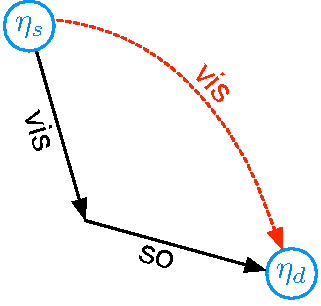
\includegraphics[scale=0.6]{../Figures/MR.pdf}
\caption{A simple way of showing contracts}
\label{fig:ctrt}
\end{figure}




\subsection{Core Algorithm Operational Semantics}
Here we explain the the core operational semantics of our algorithm, which for simplicity reasons, 
is parametrized over a single contract $\psi$:
\begin{smathpar}
\begin{array}{lcc}
\psi = \forall (a,b). a \xrightarrow{R} b  \Rightarrow a
\xrightarrow{vis} b, & \spc & R=r_1;r_2;...;r_k \\
\end{array}
\end{smathpar}
Before intorducing the semantics, let us define the inverse of a
given relation $R=r_1;r_2;...;r_k$.
The following definitions are parametrized over an execution $E$ and a set of \emph{available} effects V.
The idea is to define the inverse only if the \emph{necessary
information} about the sequence of relations, is available in V; this
way we can capture the reality of the distributed stores, where some
effects, carrying the required info about the relation being computed
might not be present at the moment.
\begin{smathpar}
\begin{array}{ccc}
   b \in (R;r_k)^{-1}_V (a) & \iff & \exists c.(c\in r_k^{-1} (a)) \wedge (b \in R^{-1}
   (c))  \wedge  (r_k^{-1}(a) \subseteq V)
\end{array}
\end{smathpar}
The above definition is based on the following definition of
the inverse of a clause :
\begin{smathpar}
r^{-1}(S) = 
\begin{cases}
\begin{array}{lll}
\bigcup^{}_{e\in S}. \{\eta|(\eta,e) \in E.r \} & if &r\in\{so,vis\} \\ 
r_1^{-1}(S)\cup r_2^{-1}(S) & if & r=r_1\cup r_2\\
G_{r}(S,\emptyset) & if &  r=r^* 
\end{array}
\end{cases}
\end{smathpar}
Where we define the helping function $G$ as follows: 
\begin{smathpar}
G_r(S,R) =
\begin{cases}
\begin{array} {lll}
G_r(r^{-1}(S,R\cup r^{-1}(S))) &if& r^{-1}(S) \neq \emptyset  \\
R  & &  otherwise
\end{array}
\end{cases}
\end{smathpar}
Given a set of effects, we also define its maximal closed subset
under the relation R as follows: 
\begin{smathpar}
\left \lfloor S \right \rfloor_V = S' \spc \mathtt{iff} \spc S'
\subseteq S \; \wedge \;
R_V^{-1}(S') \subseteq S' \; \wedge \; 
\not\exists
S''.((R_V^{-1}(S''))\subseteq S''\wedge |S''|>|S'|)
\end{smathpar}
\begin{figure}[t]
\raggedright
\textbf{Auxiliary Definitions}\\ \vspace{-2mm}
%
\begin{minipage}{0.5\textwidth}
\begin{fmathpar}
\begin{array}{lclcl}
  \multicolumn{5}{c}{
    {op} \in \mathtt{Operation\; Name} \spc \spc
    {v} \in \mathtt{Return\; Value} \spc \spc
    {s} \in \mathtt{Session\; Id} \spc\spc
  } 
  \\ 
  \eff & \in & \mathtt{Effect} & \coloneqq &  (s,op,v)\\
  F_{op} & \in & \mathtt{Op.\,Def.} & \coloneqq & \set{\eff} \mapsto v\\
  \EffSoup & \in & \mathtt{Eff\,Soup}	  & \coloneqq & \set{\eff} \\
  \visZ,\soZ &	\in & \mathtt{Relations} & \coloneqq & \set{(\eff,\eff)} \\
  {\E} 	& \in & \mathtt{Exec\;State}  & \coloneqq & \Exec \\
\end{array}
\end{fmathpar}
\end{minipage}
%

\vspace {3mm}

\textbf{Auxiliary Reduction} \; \\
\fcolorbox{black}{pgrey}{\scriptsize \(\auxred{S} {(\E,op_{<s,i>})} {} {(\E',\eff)}\)}\\
\begin{minipage}{0.9\textwidth}
\vspace{2mm}
\rulelabel{Oper}
\vspace{-2mm}
\begin{fmathpar}
\stretcharraybig
\begin{array}{l}
\RuleTwo
{
%\Theta(\rho \mapsto (v,cache)) \qquad
S \subseteq \EffSoup \qquad F_{op}(S) = v \qquad
\eta \not\in S \qquad
\eff = (s,op,v) \qquad  \\
%\id(\eta) = i \qquad
%\{\eff'\} = \EffSoup_{({\sf SessID}=s,\,{\sf SeqNo}=i-1)}\\
\EffSoup' = \EffSoup \cup \{\eff\}  \qquad
\visZ' = \visZ \cup S \times\{\eff\}\qquad
\soZ' = \soZ \cup \{(\eta',\eta) \,|\, \eta'\in \EffSoup_{({\sf
SessID}=s)}      \}\qquad
%\soZ' = (\soZ^{-1}(\eff') \cup \eff') \times\{\eff\} \cup \soZ
}
{
  \auxred {S} {((\EffSoup,\visZ,\soZ), op_{<s,i>}))}
  {} {((\EffSoup',\visZ',\soZ'),\eta)}
}
\end{array}
\end{fmathpar}
\end{minipage}
\vspace{4mm}\\
\textbf{Operational Semantics} \; \\
  \fcolorbox{black}{pgrey}{\scriptsize \((\E,op_{<s,i>}) \;\xrightarrow{V}\; (\E',\eff)\)}\\
\vspace{2mm}
\begin{minipage}{0.45\textwidth}
\rulelabel{UB Exec}
\vspace{-2mm}
\begin{fmathpar}
\stretcharraybig
\begin{array}{l}
\RuleTwo
{
  \visZ \subseteq r_k \spc
  V \subseteq E.A \spc  
  V'= \left \lfloor V \right \rfloor_V \spc
  \\ %   R^{-1}_{V}(\eta) \subseteq V' \\
  \auxred {V'} {(E, op_{<s,i>}))}
    {} {(E',\eta)} 
}
{
  (\E,op_{<s,i>}) \;\xrightarrow{V}\; (\E', \eff)
}
\end{array}
\end{fmathpar}
\end{minipage}
\hfill
\begin{minipage}{0.45\textwidth}
\rulelabel{LB Exec}
\vspace{-2mm}
\begin{fmathpar}
\stretcharraybig
\begin{array}{l}
\RuleTwo
{
     \visZ \not\subseteq r_k \spc
     V \subseteq E.A \spc  
     R^{-1}_{V}(\eta) \subseteq V \\
  \auxred {V} {(E, op_{<s,i>}))}
    {} {(E',\eta)} 
}
{
  (\E,op_{<s,i>}) \;\xrightarrow{V}\; (\E', \eff)
}
\end{array}
\end{fmathpar}
\end{minipage}
\\
\vspace{5mm}
\hrulefill\\
\caption{Core Operational semantics of a replicated data store.}
\label{fig:semantics}
\end{figure}


\newpage




\subsection {Shim Layer Operational Semantics}
In this section we introduce the complete behavior of our multi-consistenct shim layer as a new set of operational semantics. 
The rules are parametrized over a given map of operation names to
contracts, $\Psi :  op
\mapsto \psi $ and we assume each contract is of the form:
$\Psi(op)=\forall (a,b). a \xrightarrow{Q_{op}} \Rightarrow a \xrightarrow{vis} b.$ 
We use $Q_{op}[m]$ notation to refer to the m'th clause in the composition.
We define a pool to be a set of effects and a value that contains all
the effects that arrive to the replica. 
Our shim layer, also maintains a set of k caches (one cache for each
given contract). Each cache is maintained to be the largest
subset of pool that is closed under its
contract.  i.e. $\forall \eff \in \Cache(op). Q_{op}^{-1}(\eff)
\subseteq \Cache(op) $ 
\\We also maintain a level of availability for each effect
according to an operation and the current pool. If the availability of an effect for
$op$ is $x$, it means
that the effect satisfies the suffix of size $x$ of contract $\Psi(op)$.
An effect $\eta$ satisfies a suffix of size $x\geq 1$ of contaract
$\psi=\forall (a,b). a \xrightarrow{q_1;q_2;...;q_n} b$,
written as $ (\eta \models_{\Pool}^{x} \psi )$, if and only if
$(q_{n-(x-1)};...;q_{n} )^{-1}_{\Pool}(\{\eta\}) \subseteq \Pool$. The
initial availability value for all effects is 0, and increases when more
dependent effects arrive. 
\\
Following are the formal definitions: 
\\
\begin{minipage}{\columnwidth}
\begin{smathpar}
\stretcharraybig
\begin{array}{lclcl}
  \multicolumn{5}{c}{
    {\delta} \in \mathtt{Replicated\; Data\; Type} \spc\spc
    {v} \in \mathtt{Value}\spc\spc
    {op} \in \mathtt{Operation\; Name}
  }\\
  \multicolumn{5}{c}{
    {s} \in \mathtt{Session\; Id} \spc\spc
    {i} \in \mathtt{Effect\; Id} \spc\spc
    {\rho} \in \mathtt{Replica\; Id}
  }\\
  \eff & \in & \mathtt{Effect} & \coloneqq &  (s,i,op,v)\\
   {\Pool} & \in & \mathtt {Pool} & \coloneqq & (v,\set {\eff}) \\
   {\Cache} & \in & \mathtt {Cache} & \coloneqq & op \mapsto (v,\set{\eff})\\
   \Avail & \in & \mathtt {Avail} & \coloneqq & op \mapsto (\eff \mapsto
\{0,1,...,k-1\}) \\
  F_{op} & \in & \mathtt{Op.\,Def.} & \coloneqq & v \rightarrow \eta\\
  \EffSoup & \in & \mathtt{Eff\,Soup}	  & \coloneqq & \set{\eff} \\
  \visZ,\soZ &	\in & \mathtt{Relations} & \coloneqq & \set{(\eff,\eff)} \\
  {\E} 		& \in & \mathtt{Exec\;State}  & \coloneqq & \Exec \\
  \Theta  & \in & \mathtt{Store}      & \coloneqq & \rho \mapsto
  (\Pool, {\Cache}, \Avail) \\
  {\sigma} 	& \in & \mathtt{Session} 					 	& \coloneqq & \cdot \ALT op::\sigma \\
  \Sigma 		& \in & \mathtt{Session\;Soup}   	 	& \coloneqq &
        \langle s, i, \sigma \rangle \pll \Sigma \ALT \emptyset \\
\end{array}
\end{smathpar}
\end{minipage}
%
\begin{smathpar}
\begin{array}{c}
\ssn(s,\_,\_,\_) = s \spc\spc
\id(\_,j,\_,\_) = j \spc\spc
\oper(\_,\_,op,\_) = op \spc\spc
\rval(\_,\_,\_,n) = n\\
\end{array}
\end{smathpar}



\begin{figure*}[h]
\raggedright
%

\textbf{Auxiliary Definitions}\\
%
\begin{minipage}{\columnwidth}
\begin{smathpar}
\stretcharraybig
\begin{array}{lclcl}
  \multicolumn{5}{c}{
    {\delta} \in \mathtt{Replicated\; Data\; Type} \spc\spc
    {v} \in \mathtt{Value}\spc\spc
    {op} \in \mathtt{Operation\; Name}
  }\\
  \multicolumn{5}{c}{
    {s} \in \mathtt{Session\; Id} \spc\spc
    {i} \in \mathtt{Effect\; Id} \spc\spc
    {\rho} \in \mathtt{Replica\; Id}
  }\\
  \eff & \in & \mathtt{Effect} & \coloneqq &  (s,i,op,v)\\
   {\Pool} & \in & \mathtt {Pool} & \coloneqq & (v,\set {\eff}) \\
   {\Cache} & \in & \mathtt {Cache} & \coloneqq & (v,\set{\eff})\\
  F_{op} & \in & \mathtt{Op.\,Def.} & \coloneqq & v \rightarrow \eta\\
  \EffSoup & \in & \mathtt{Eff\,Soup}	  & \coloneqq & \set{\eff} \\
  \visZ,\soZ &	\in & \mathtt{Relations} & \coloneqq & \set{(\eff,\eff)} \\
  {\E} 		& \in & \mathtt{Exec\;State}  & \coloneqq & \Exec \\
  \Theta  & \in & \mathtt{Store}      & \coloneqq & \rho \mapsto (\Pool,\Cache) \\
  {\sigma} 	& \in & \mathtt{Session} 					 	& \coloneqq & \cdot \ALT op::\sigma \\
  \Sigma 		& \in & \mathtt{Session\;Soup}   	 	& \coloneqq &
        \langle s, i, \sigma \rangle \pll \Sigma \ALT \emptyset \\
\end{array}
\end{smathpar}
\end{minipage}
%

\begin{smathpar}
\begin{array}{c}
\ssn(s,\_,\_,\_) = s \spc\spc
\id(\_,j,\_,\_) = j \spc\spc
\oper(\_,\_,op,\_) = op \spc\spc
\rval(\_,\_,\_,n) = n\\
\end{array}
\end{smathpar}

\vspace{5mm}
\textbf{Auxiliary Reduction} \;
  \fbox{\(\auxred{v} {(\E,\langle s,i,op \rangle)} {} {(\E',\eff)}\)}\\

\begin{minipage}{\textwidth}
\rulelabel{Oper}
\begin{smathpar}
\stretcharraybig
\begin{array}{l}
\RuleTwo
{
%\Theta(\rho \mapsto (v,cache)) \qquad
F_{op}(v) = \eta \qquad
\ssn(\eta) = s \qquad 
\id(\eta) = i \qquad
%\{\eff'\} = \EffSoup_{({\sf SessID}=s,\,{\sf SeqNo}=i-1)}\\
\EffSoup' = \EffSoup \cup \{\eff\} \\
\visZ' = \visZ \cup S \times\{\eff\}\qquad
\soZ' = \soZ \cup \{(\eta',\eta) \,|\, \eta'\in \EffSoup \conj 
    \ssn(\eta')=s \conj \id(\eta')<i\}\qquad
%\soZ' = (\soZ^{-1}(\eff') \cup \eff') \times\{\eff\} \cup \soZ
}
{
  \auxred {v} {((\EffSoup,\visZ,\soZ), \langle s,i,op \rangle}
  {} {((\EffSoup',\visZ',\soZ'),\eta)}
}
\end{array}
\end{smathpar}
\end{minipage}


\vspace{5mm}
\textbf{Operational Semantics} \;
  \fbox{\((\E,\Theta,\Sigma) \;\xrightarrow{\eff}\; (\E',\Theta',\Sigma')\)}\\

\begin{minipage}{3in}
\rulelabel{Pool Refresh}
\begin{smathpar}
\stretcharraybig
\begin{array}{l}
\RuleTwo
{ 
  \eta \in \E.\EffSoup \spc
  \Theta(\rho) = (\Pool,\Cache) \spc
  \eta \not\in \Pool_e \\
  \Pool' = (apply \; \eta\; \Pool_v,\Pool_e \cup \{\eta\}) \spc \\
  \Theta' = \Theta[\rho \mapsto (\Pool',\Cache)]\\
}
{
  (\E,\Theta,\Sigma) \;\xrightarrow{\eff}\; (\E, \Theta', \Sigma)
}
\end{array}
\end{smathpar}
\end{minipage}

\vspace{5mm}
\begin{minipage}{2.8in}
\rulelabel{Cache Refresh}
\begin{smathpar}
\stretcharraybig
\begin{array}{l}
\RuleTwo
{
  \Theta(\rho) = (\Pool,\Cache) \spc \eta \in \Pool_e
  \\ \eta \not\in \Cache_e \spc
  \Cache'=(apply \; \eta \; \Cache_v ,\Cache_e \cup \{\eta\}) \\ \psi^{-1}
  (\eta) \subseteq \Cache_e
 \spc  \Theta' = \Theta[\rho \mapsto (\Pool,\Cache')]\\
}
{
  (\E,\Theta,\Sigma) \;\xrightarrow{\eff}\; (\E, \Theta', \Sigma)
}
\end{array}
\end{smathpar}
\end{minipage}
\hspace{12 mm}
\vspace{3mm}
\begin{minipage}{2.3in}
\rulelabel{Exec}
\begin{smathpar}
\stretcharraybig
\begin{array}{l}
\RuleTwo
{
  \auxred{\CacheFinder_{\psi}(\Theta(\rho))} {(\E,\langle s,i,op \rangle)} {} {(\E',\eta)}  \\
  \Theta(\rho) = (\Pool,\Cache) \spc \psi^{-1}(\eta) \subseteq \Pool_e  \spc
}
{
  (\E,\Theta,\langle s,i,op::\sigma \rangle \pll \Sigma) 
    \;\xrightarrow{\eff}\;
  (\E',\Theta,\langle s,i+1,\sigma \rangle \pll \Sigma) 
}
\end{array}
\end{smathpar}
\end{minipage}


\caption{Operational semantics of a replicated data store.}
\label{sem:oper}
\end{figure*}









%================================ SECTION FIVE








%% Acknowledgments
%\begin{acks}                            %% acks environment is optional
                                        %% contents suppressed with 'anonymous'
  %% Commands \grantsponsor{<sponsorID>}{<name>}{<url>} and
  %% \grantnum[<url>]{<sponsorID>}{<number>} should be used to
  %% acknowledge financial support and will be used by metadata
  %% extraction tools.
%  This material is based upon work supported by the
%  \grantsponsor{GS100000001}{National Science
%    Foundation}{http://dx.doi.org/10.13039/100000001} under Grant
%  No.~\grantnum{GS100000001}{nnnnnnn} and Grant
%  No.~\grantnum{GS100000001}{mmmmmmm}.  Any opinions, findings, and
%  conclusions or recommendations expressed in this material are those
%  of the author and do not necessarily reflect the views of the
%  National Science Foundation.
%\end{acks}


%% Bibliography
%\bibliography{bibfile}


%% Appendix
%\appendix
%\section{Appendix}

%Text of appendix \ldots

\end{document}
